\documentclass{article}

\usepackage[a4paper,margin=2cm]{geometry}
\usepackage{amsmath}
\usepackage{amsfonts}
\usepackage{fancyhdr}
\usepackage{hyperref}
\usepackage{graphicx}
\usepackage{subcaption}

\title{COMP20008 Assignment 2 \\Question 2 - Report}
\date{\today}
\author{Lucas Fern (1080613)}

\begin{document}
\maketitle
Both tasks 2A and B started with record linkage of the the datasets in \verb|world.csv| and \verb|life.csv| using the intersection of country codes. This was so that only records that had an attached life expectancy classification were present. The records were then split into training and testing sets with sizes $\frac{2}{3}$ and $\frac{1}{3}$ respectively using the life expectancies as class labels. The missing values in \verb|world.csv| were imputed to be the median of the values for that feature. This was done separately on the training and testing data in order to avoid the data selected for testing having any influence over the training set.
\section*{Task 2A}
In task 2A the k-NN algorithm performed classification more effectively than the decision tree. The results for the algorithms were:
\begin{verbatim}
    Accuracy of decision tree: 0.721 (Maximum accuracy recorded)
    Accuracy of k-nn (k=5): 0.820
    Accuracy of k-nn (k=10): 0.869
\end{verbatim}
Though the accuracy of the decision tree relies on a random seed and hence was not perfectly consistent over all trials.\\[2mm]
The k-NN algorithm was superior for both \verb|k=5| and \verb|k=10|, but \verb|k=10| achieved the best accuracy. This makes sense due to the reasonably large size of the dataset, since increasing the amount of neighbours will increase the amount of data points contributing to each country's classification without forcing it to consider data points at too significant of a distance.
\section*{Task 2B}
In task 2B feature engineering was implemented with Principal Component Analysis (PCA) in an attempt to improve the performance of the 5-NN algorithm on classification of life expectancies. After record linkage, splitting, and imputation, interaction term pairs were generated for the 190 combinations of features by pairwise multiplication of the values in the columns, these were recorded as new features.\\[2mm]
The data was then standardised to have a mean of zero and unit variance so that Euclidean distance would not be significantly different between any combination of features. This is the reason the standardisation occurred before performing k-Means clustering, as otherwise the resulting clustering was very unbalanced.\\[2mm]
Visual assessment of clustering tendency was then performed to inform a decision as to the amount of clusters to be used in generating the final feature. The results of this are shown in fig. \ref{fig:VAT}, where \ref{fig:VAT}b shows where I believe distinctions may lie between clusters. 
\begin{figure}[!ht]
    \centering
    \begin{subfigure}[b]{0.45\linewidth}
      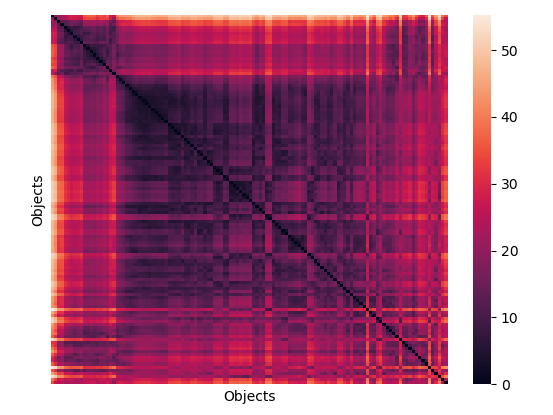
\includegraphics[width=\linewidth]{task2b-VAT.png}
      \caption{VAT of the training data.}
    \end{subfigure}
    \begin{subfigure}[b]{0.45\linewidth}
      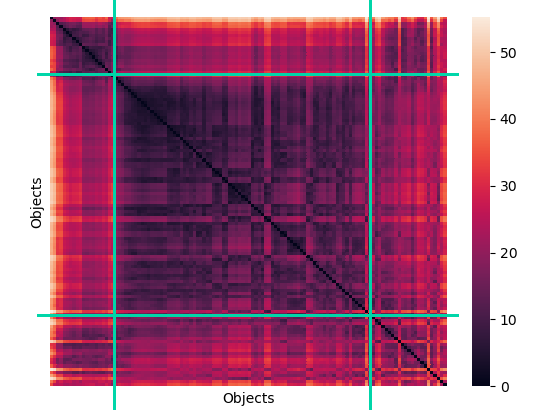
\includegraphics[width=\linewidth]{task2b-VAT-annotated.png}
      \caption{Annotated to show possible clusters.}
    \end{subfigure}
    \caption{Visual assessment of the Clustering Tendency of the Training `World' Data.}
    \label{fig:VAT}
\end{figure}
Based on this visual assessment, 3 centroids were chosen for clustering, which is further justified by the fact that this is the amount of options a country's life expectancy has to be categorised into. In the last step before feature selection, points in the testing dataset were assigned to a cluster based on the centroid with minimum Euclidean distance.

\subsection*{Feature Section}
The 5-NN algorithm was run on 3 different combinations of features in this task. The simplest combination was to simply take the first 4 columns of the features. 5-NN classification with this selection yielded an accuracy of 0.754.\\[2mm]
Feature selection was also done with Principal Component Analysis by transforming the data with\\\verb|sklearn.decomposition.PCA()| using \verb|n_components=4|. The same transformation was applied to the test set and running 5-NN classification with these four features gave an accuracy of 0.770, slightly higher than previous though lower than when considering every feature individually in task 2A.\\[2mm]
The final feature selection method was to select four based on which yielded the greatest improvement to the classification accuracy and made intuitive sense to me based on the nature of the data. The selected features were: \begin{verbatim}
    (1) Cause of death, by non-communicable diseases (% of total)
    (2) Maternal mortality ratio (modeled estimate, per 100,000 live births)
    (3) Mortality from CVD, cancer, diabetes or CRD between exact ages 30 and 70, female (%)
\end{verbatim}
and the product of\begin{verbatim}
    (4) Access to electricity, rural (% of rural population), and
        Birth rate, crude (per 1,000 people).
\end{verbatim}
I believe \verb|(1)| is a good indicator of life expectancy as we might expect a correlation between an aging population and an increase in death by non-communicable diseases as communicable diseases become more treatable and people in high income countries see causes of death such as cancer and heart failure increasing as a result. Feature \verb|(2)| is not only a measure of deaths of mothers at child bearing (younger) ages, but may also indicate a larger underlying issue of poor healthcare in a country, hence it is a good indicator. Similarly to feature \verb|(1)|, feature \verb|(3)| is a measure of deaths to specific non-communicable diseases, with the added effect that similarly to feature \verb|(2)| it is also a direct measure of mortality in people of younger ages. Finally, both individual features that combine to make feature \verb|(4)| are strong indicators of the level of development of a country, where a developing country often has a much higher birth rate and lower access to electricity. Hence I believe these combine to effectively predict developing countries that may have lower life expectancies.\\[2mm]
This feature selection produced the best classification results of all at an accuracy of 0.902. It is unsurprising that this method produces better results than simply selecting the first four features, as there is no justification behind that selection. It is somewhat more surprising that it outperformed PCA, though a possible explanation for the relatively low score of feature selection through PCA is that the linear combination of features that PCA found did not capture a complex non-linear relationship that relates the features to the class label.
\subsection*{Evaluation/Comments}
I consider the model to be relatively accurate but far from perfect. Although it would be good to have complete datasets for every single country, the data provided was already relatively close to complete and it would be unreasonable to expect a very significant improvement to the performance of my algorithm by adding data from the 22 countries missing from the intersection of the datasets. The accuracies seen - especially for 10-NN classification in task 2A and with my feature selection in 2B - seem relatively good, hence my assessment of decent accuracy.\\[2mm]
The results may be further improved by engineering other features such as one as the result of a hierarchical agglomerative clustering or though other combinations than pairwise multiplication. Features may also be selected using more scientifically rigorous methods such as the $\chi^2$ test to determine dependence.
\end{document}